Mediante l'oscilloscopio, verificare la funzione di trasferimento per filtri passa basso, passa banda e reiezione di banda.\begin{wrapfigure}[6]{r}[0pt]{130mm}
	\centering
    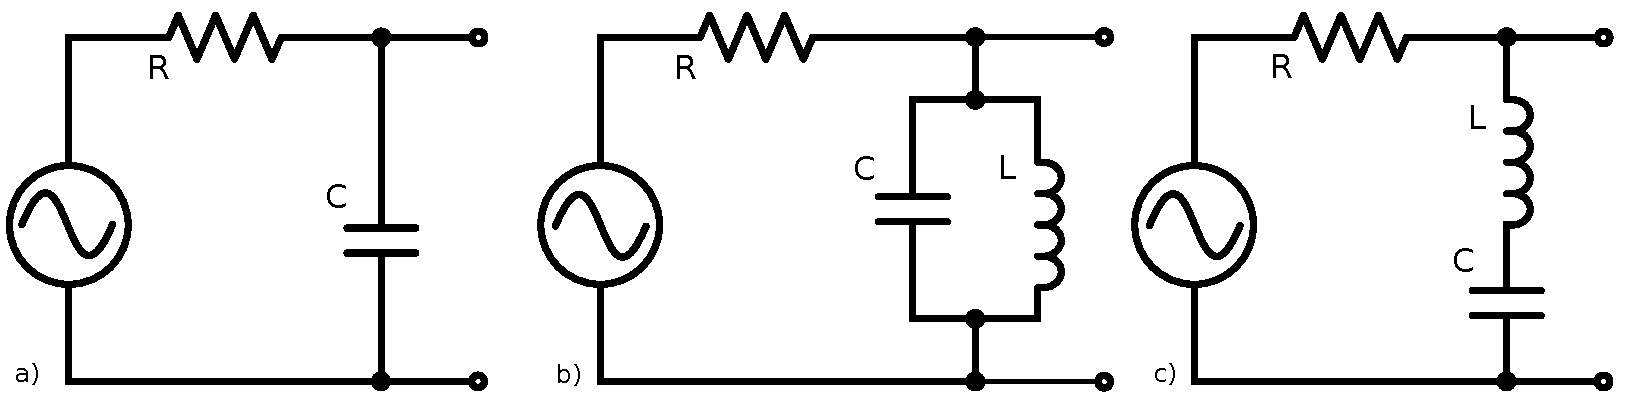
\includegraphics[width=0.7\textwidth]{circuiti.pdf}
    \caption{Schema dei circuiti utilizzati: a) filtro passa basso; b) filtro passa banda; c) filtro a reiezione di banda}
    \label{fig:circuito}
\end{wrapfigure}

\section{Strumenti}

$\bullet \quad$Oscilloscopio \\
$\bullet \quad$Cablaggio\\
$\bullet \quad$Breadboard (basetta sperimentale)\\
$\bullet \quad$Generatore di forme d'onda\\
$\bullet \quad$Multimetro digitale\\
$\bullet \quad$Decadi di resistenze,\\
\hspace{20pt} capacitori e induttanze\\
